\appendix
\section{Data}
\begin{table}[h]
\caption{Item-level matrices used (OLL: Open LLM Leaderboard v2; HELM). ``const.\ items'': items answered identically by all models. Accuracy statistics are over models.}
\label{tab:data}
\centering\scriptsize\begin{tabular}{llrrrrrr}
\toprule
benchmark & source & models & items & mean acc. & sd acc. & range & const.\ items \\
\midrule
arc challenge & OLL & 218 & 1172 & 52.2 & 12.9 & 20.5--75.1 & 32 \\
bbh & OLL & 446 & 5761 & 44.7 & 11.6 & 24.1--74.7 & 0 \\
gpqa & OLL & 447 & 1192 & 28.9 & 3.8 & 22.5--43.7 & 0 \\
ifeval & OLL & 448 & 541 & 33.3 & 20.4 & 3.7--88.0 & 7 \\
mmlu pro & OLL & 448 & 12032 & 28.1 & 12.9 & 10.3--59.7 & 1 \\
musr & OLL & 448 & 756 & 39.9 & 4.1 & 32.3--53.6 & 10 \\
openllm math & OLL & 447 & 894 & 5.1 & 6.8 & 0.0--35.6 & 119 \\
commonsense & HELM & 83 & 500 & 82.3 & 17.3 & 22.2--97.2 & 0 \\
gsm & HELM & 83 & 1000 & 65.7 & 24.9 & 2.8--95.6 & 3 \\
legalbench & HELM & 79 & 2047 & 53.3 & 10.6 & 22.8--70.2 & 53 \\
math & HELM & 83 & 437 & 56.8 & 27.4 & 2.5--93.4 & 1 \\
med qa & HELM & 83 & 1000 & 59.4 & 16.4 & 21.5--86.9 & 2 \\
mmlu & HELM & 83 & 567 & 61.3 & 12.4 & 22.9--81.1 & 1 \\
\bottomrule
\end{tabular}

\end{table}
\begin{table}[h]
\caption{Absolute RMSE (accuracy points; $\sqrt{\text{seed-averaged MSE}}$) at $n=100$ for random splits and stronger targets.}
\label{tab:abs}
\centering\tiny\setlength{\tabcolsep}{2pt}\begin{tabular}{llrrrrrrrrrrrrr}
\toprule
split & method & arc challenge & bbh & commonsense & gpqa & gsm & ifeval & legalbench & math & med qa & mmlu & mmlu pro & musr & openllm math \\
\midrule
random & Random sampling & 4.4 & 4.6 & 3.1 & 4.2 & 3.9 & 3.8 & 4.8 & 3.5 & 4.7 & 4.0 & 4.1 & 4.1 & 1.9 \\
random & Difficulty-stratified sampling & 3.3 & 4.1 & 2.4 & 4.1 & 3.3 & 3.2 & 3.5 & 3.0 & 3.7 & 3.0 & 3.5 & 3.6 & 1.7 \\
random & Random + IRT-AIPW & 3.1 & 3.7 & 2.7 & 3.7 & 3.2 & 3.0 & 3.4 & 3.0 & 3.5 & 3.1 & 3.3 & 3.2 & 1.7 \\
random & VA-PPS + Cal-IRT (ours) & 2.8 & 3.5 & 2.5 & 3.5 & 3.1 & 2.9 & 3.3 & 3.2 & 3.5 & 2.9 & 3.1 & 2.8 & 1.3 \\
random & VA-PPS + ShrinkCal-IRT (ours) & 2.5 & 3.0 & 2.6 & 3.0 & 3.3 & 2.8 & 3.3 & 3.3 & 3.5 & 2.9 & 2.8 & 2.4 & 1.3 \\
top & Random sampling & 4.4 & 4.6 & 1.9 & 4.5 & 2.7 & 4.0 & 5.0 & 3.0 & 4.3 & 3.9 & 4.5 & 4.1 & 3.3 \\
top & Difficulty-stratified sampling & 3.2 & 4.0 & 1.6 & 3.9 & 2.4 & 3.7 & 3.4 & 2.4 & 3.0 & 2.9 & 4.0 & 3.8 & 3.0 \\
top & Random + IRT-AIPW & 2.9 & 4.0 & 1.8 & 4.1 & 2.3 & 3.5 & 3.3 & 2.7 & 3.2 & 2.8 & 4.1 & 3.2 & 3.0 \\
top & VA-PPS + Cal-IRT (ours) & 2.8 & 3.6 & 1.3 & 3.8 & 2.3 & 3.5 & 2.9 & 2.3 & 3.4 & 2.5 & 4.1 & 3.0 & 2.8 \\
top & VA-PPS + ShrinkCal-IRT (ours) & 3.2 & 4.0 & 1.8 & 4.1 & 2.7 & 3.8 & 3.4 & 2.8 & 3.9 & 3.1 & 4.4 & 3.3 & 3.2 \\
\bottomrule
\end{tabular}

\end{table}

\section{Implementation details}\label{app:impl}
\textbf{IRT.} $P(y_{ji}=1)=\sigma(\theta_j^\top\alpha_i+\beta_i)$, minimised over $(\theta,\alpha,\beta)$ with scipy L-BFGS-B (max.\ 150 iterations, 20 correction pairs, float32 matrix products) on the sum of binary cross-entropies plus $\frac12\|\theta\|^2+\frac12\|\alpha\|^2+0.05\|\beta-\beta^{0}\|^2$, where $\beta^{0}_i=\mathrm{logit}(\mathrm{clip}(\bar p_i,0.02,0.98))$ and initial $\theta,\alpha\sim 0.1\,\mathcal N(0,I)$. Target ability: MAP with prior $\mathcal N(0,4I)$ by batched damped Newton iterations (step clipped to $\pm2$, at most 25 iterations). Platt recalibration: two-parameter Newton (at most 20 iterations, steps clipped to $\pm1$) on the coreset, ridge penalty 1 towards $(s,c)=(1,0)$. ShrinkCal: $\hat v_t=\mathrm{Var}_C(y-\hat p)/n\cdot(1-n/N)$ (unbiased sample variance), $c_0=0.5$.\\
\textbf{VA-PPS.} $v_i$ is the mean squared residual of the $d=4$ IRT fit on the source models; $s_i=\sqrt{\max(v_i,10^{-4})}$; inclusion probabilities by water-filling to $\sum\pi_i=n$; systematic sampling over difficulty-sorted items (ties broken at random) with a uniformly random start.\\
\textbf{Anchor points.} scikit-learn \texttt{KMeans} with $k=n$, \texttt{n\_init}=1, \texttt{max\_iter}=30 on the source item vectors; the item closest to each centroid is the anchor, weight = cluster size$/N$.\\
\textbf{D-optimal.} Greedy $\log\det$ maximisation of $I+\sum_i \bar w_i\alpha_i\alpha_i^\top$ with $\bar w_i=\overline{p(1-p)}$ over source models, via Sherman--Morrison updates.\\
\textbf{Ridge.} \texttt{RidgeCV}, $\alpha\in\{10^{-2},\dots,10^{3}\}$ (12 values), source coreset responses $\to$ source full accuracy.\\
\textbf{Cross-fitting.} 5 folds over coreset items.\\
\textbf{AUTO.} Inner splits use seed-dependent random permutations; 2 repetitions of coreset draws per inner split; inner IRT fits are refitted on the inner source subset.

\section{Additional results}
\begin{table}[h]
\caption{Relative RMSE at all five budgets (same format as Table~\ref{tab:main}); columns are protocol$\times n$ in the order $n=10,25,50,100,200$.}\label{tab:full}
\centering\tiny\setlength{\tabcolsep}{1.5pt}\resizebox{\linewidth}{!}{\begin{tabular}{lccccccccccccccc}
\toprule
 & \multicolumn{5}{c}{Random split} & \multicolumn{5}{c}{Held-out organisations} & \multicolumn{5}{c}{Stronger targets (extrapolation)} \\
 & $n$=10 & $n$=25 & $n$=50 & $n$=100 & $n$=200 & $n$=10 & $n$=25 & $n$=50 & $n$=100 & $n$=200 & $n$=10 & $n$=25 & $n$=50 & $n$=100 & $n$=200 \\
\midrule
Random sampling & 1.00\,\scriptsize(1.00--1.00) & 1.00\,\scriptsize(1.00--1.00) & 1.00\,\scriptsize(1.00--1.00) & 1.00\,\scriptsize(1.00--1.00) & 1.00\,\scriptsize(1.00--1.00) & 1.00\,\scriptsize(1.00--1.00) & 1.00\,\scriptsize(1.00--1.00) & 1.00\,\scriptsize(1.00--1.00) & 1.00\,\scriptsize(1.00--1.00) & 1.00\,\scriptsize(1.00--1.00) & 1.00\,\scriptsize(1.00--1.00) & 1.00\,\scriptsize(1.00--1.00) & 1.00\,\scriptsize(1.00--1.00) & 1.00\,\scriptsize(1.00--1.00) & 1.00\,\scriptsize(1.00--1.00) \\
Difficulty-stratified sampling & 0.84\,\scriptsize(0.79--0.88) & 0.83\,\scriptsize(0.79--0.88) & 0.83\,\scriptsize(0.79--0.87) & 0.83\,\scriptsize(0.79--0.87) & 0.84\,\scriptsize(0.80--0.88) & 0.83\,\scriptsize(0.76--0.91) & 0.83\,\scriptsize(0.76--0.89) & 0.83\,\scriptsize(0.77--0.89) & 0.86\,\scriptsize(0.80--0.91) & 0.84\,\scriptsize(0.79--0.89) & 0.85\,\scriptsize(0.80--0.92) & 0.82\,\scriptsize(0.78--0.87) & 0.83\,\scriptsize(0.78--0.88) & 0.82\,\scriptsize(0.78--0.87) & 0.82\,\scriptsize(0.78--0.86) \\
Random + linear calibration & 0.56\,\scriptsize(0.45--0.68) & 0.67\,\scriptsize(0.57--0.76) & 0.73\,\scriptsize(0.65--0.80) & 0.79\,\scriptsize(0.74--0.83) & 0.81\,\scriptsize(0.76--0.85) & 0.48\,\scriptsize(0.35--0.65) & 0.61\,\scriptsize(0.49--0.75) & 0.68\,\scriptsize(0.58--0.81) & 0.77\,\scriptsize(0.69--0.85) & 0.79\,\scriptsize(0.73--0.84) & 0.85\,\scriptsize(0.72--1.00) & 0.95\,\scriptsize(0.85--1.07) & 1.01\,\scriptsize(0.90--1.15) & 1.07\,\scriptsize(0.95--1.19) & 1.06\,\scriptsize(0.97--1.18) \\
Random + ridge regression & 0.52\,\scriptsize(0.41--0.64) & 0.61\,\scriptsize(0.50--0.72) & 0.66\,\scriptsize(0.55--0.78) & 0.73\,\scriptsize(0.63--0.83) & 0.79\,\scriptsize(0.68--0.91) & 0.43\,\scriptsize(0.32--0.60) & 0.53\,\scriptsize(0.41--0.67) & 0.57\,\scriptsize(0.46--0.73) & 0.67\,\scriptsize(0.56--0.81) & 0.71\,\scriptsize(0.62--0.85) & 0.91\,\scriptsize(0.73--1.11) & 1.12\,\scriptsize(0.94--1.32) & 1.35\,\scriptsize(1.13--1.61) & 1.65\,\scriptsize(1.37--1.96) & 2.06\,\scriptsize(1.68--2.52) \\
Anchor points (weighted mean) & 0.68\,\scriptsize(0.60--0.76) & 0.78\,\scriptsize(0.68--0.89) & 0.91\,\scriptsize(0.79--1.06) & 1.08\,\scriptsize(0.91--1.28) & 1.28\,\scriptsize(1.09--1.53) & 0.67\,\scriptsize(0.55--0.81) & 0.82\,\scriptsize(0.67--1.03) & 0.94\,\scriptsize(0.76--1.23) & 1.21\,\scriptsize(0.95--1.63) & 1.41\,\scriptsize(1.09--1.87) & 0.72\,\scriptsize(0.56--1.00) & 0.90\,\scriptsize(0.65--1.30) & 1.08\,\scriptsize(0.76--1.62) & 1.34\,\scriptsize(0.90--2.07) & 1.67\,\scriptsize(1.06--2.62) \\
Anchor points + IRT (tinyBenchmarks-style) & 0.47\,\scriptsize(0.37--0.59) & 0.58\,\scriptsize(0.47--0.71) & 0.68\,\scriptsize(0.54--0.85) & 0.83\,\scriptsize(0.66--1.07) & 1.00\,\scriptsize(0.78--1.33) & 0.38\,\scriptsize(0.31--0.48) & 0.48\,\scriptsize(0.40--0.58) & 0.54\,\scriptsize(0.46--0.65) & 0.67\,\scriptsize(0.58--0.81) & 0.77\,\scriptsize(0.66--0.88) & 0.80\,\scriptsize(0.63--0.99) & 1.02\,\scriptsize(0.85--1.22) & 1.22\,\scriptsize(1.03--1.43) & 1.40\,\scriptsize(1.11--1.73) & 1.52\,\scriptsize(1.08--2.05) \\
D-optimal items + IRT (info-based) & 0.56\,\scriptsize(0.43--0.73) & 0.70\,\scriptsize(0.55--0.92) & 0.83\,\scriptsize(0.64--1.10) & 1.01\,\scriptsize(0.79--1.33) & 1.19\,\scriptsize(0.92--1.59) & 0.43\,\scriptsize(0.32--0.55) & 0.53\,\scriptsize(0.41--0.67) & 0.61\,\scriptsize(0.48--0.76) & 0.77\,\scriptsize(0.63--0.96) & 0.89\,\scriptsize(0.73--1.09) & 0.77\,\scriptsize(0.62--0.96) & 1.01\,\scriptsize(0.85--1.20) & 1.28\,\scriptsize(1.07--1.53) & 1.62\,\scriptsize(1.33--1.98) & 2.00\,\scriptsize(1.58--2.55) \\
Random + IRT (pure) & 0.56\,\scriptsize(0.46--0.67) & 0.65\,\scriptsize(0.55--0.75) & 0.69\,\scriptsize(0.60--0.80) & 0.78\,\scriptsize(0.70--0.86) & 0.91\,\scriptsize(0.81--1.02) & 0.48\,\scriptsize(0.37--0.61) & 0.57\,\scriptsize(0.46--0.69) & 0.61\,\scriptsize(0.52--0.73) & 0.71\,\scriptsize(0.64--0.80) & 0.81\,\scriptsize(0.76--0.87) & 0.92\,\scriptsize(0.72--1.14) & 1.08\,\scriptsize(0.90--1.29) & 1.25\,\scriptsize(1.08--1.46) & 1.54\,\scriptsize(1.35--1.79) & 2.05\,\scriptsize(1.76--2.42) \\
Random + IRT-AIPW & 0.73\,\scriptsize(0.68--0.79) & 0.78\,\scriptsize(0.73--0.82) & 0.78\,\scriptsize(0.74--0.83) & 0.80\,\scriptsize(0.77--0.83) & 0.78\,\scriptsize(0.74--0.82) & 0.70\,\scriptsize(0.63--0.77) & 0.77\,\scriptsize(0.71--0.83) & 0.78\,\scriptsize(0.71--0.84) & 0.80\,\scriptsize(0.74--0.86) & 0.78\,\scriptsize(0.73--0.83) & 0.74\,\scriptsize(0.68--0.81) & 0.78\,\scriptsize(0.73--0.84) & 0.79\,\scriptsize(0.73--0.84) & 0.82\,\scriptsize(0.77--0.87) & 0.83\,\scriptsize(0.78--0.88) \\
VA-PPS + IRT-AIPW & 0.74\,\scriptsize(0.68--0.81) & 0.78\,\scriptsize(0.72--0.87) & 0.80\,\scriptsize(0.74--0.87) & 0.82\,\scriptsize(0.77--0.89) & 0.80\,\scriptsize(0.74--0.89) & 0.71\,\scriptsize(0.63--0.81) & 0.75\,\scriptsize(0.68--0.83) & 0.74\,\scriptsize(0.68--0.80) & 0.77\,\scriptsize(0.71--0.82) & 0.76\,\scriptsize(0.71--0.82) & 0.72\,\scriptsize(0.65--0.80) & 0.76\,\scriptsize(0.69--0.84) & 0.80\,\scriptsize(0.72--0.89) & 0.88\,\scriptsize(0.78--0.98) & 0.84\,\scriptsize(0.73--0.96) \\
VA-PPS + IRT (pure) & 0.55\,\scriptsize(0.45--0.67) & 0.65\,\scriptsize(0.54--0.79) & 0.71\,\scriptsize(0.60--0.85) & 0.82\,\scriptsize(0.69--1.00) & 0.98\,\scriptsize(0.81--1.23) & 0.46\,\scriptsize(0.36--0.58) & 0.54\,\scriptsize(0.45--0.64) & 0.59\,\scriptsize(0.51--0.68) & 0.69\,\scriptsize(0.64--0.76) & 0.79\,\scriptsize(0.74--0.85) & 0.85\,\scriptsize(0.68--1.07) & 1.02\,\scriptsize(0.86--1.20) & 1.20\,\scriptsize(1.04--1.40) & 1.51\,\scriptsize(1.30--1.76) & 1.99\,\scriptsize(1.71--2.35) \\
VA-PPS + Cal-IRT (ours) & 0.61\,\scriptsize(0.54--0.68) & 0.69\,\scriptsize(0.63--0.75) & 0.71\,\scriptsize(0.67--0.77) & 0.75\,\scriptsize(0.71--0.80) & 0.74\,\scriptsize(0.68--0.80) & 0.56\,\scriptsize(0.47--0.64) & 0.65\,\scriptsize(0.59--0.72) & 0.69\,\scriptsize(0.62--0.76) & 0.74\,\scriptsize(0.69--0.80) & 0.73\,\scriptsize(0.66--0.79) & 0.68\,\scriptsize(0.60--0.77) & 0.70\,\scriptsize(0.64--0.76) & 0.72\,\scriptsize(0.67--0.79) & 0.76\,\scriptsize(0.70--0.82) & 0.74\,\scriptsize(0.66--0.82) \\
VA-PPS + ShrinkCal-IRT (ours) & 0.57\,\scriptsize(0.50--0.66) & 0.64\,\scriptsize(0.58--0.72) & 0.67\,\scriptsize(0.61--0.74) & 0.71\,\scriptsize(0.66--0.77) & 0.73\,\scriptsize(0.67--0.80) & 0.50\,\scriptsize(0.41--0.59) & 0.58\,\scriptsize(0.51--0.65) & 0.62\,\scriptsize(0.54--0.69) & 0.68\,\scriptsize(0.62--0.74) & 0.69\,\scriptsize(0.64--0.75) & 0.74\,\scriptsize(0.62--0.87) & 0.80\,\scriptsize(0.71--0.90) & 0.84\,\scriptsize(0.76--0.92) & 0.88\,\scriptsize(0.82--0.93) & 0.84\,\scriptsize(0.78--0.91) \\
AUTO (pseudo-shift, minimax) & 0.58\,\scriptsize(0.48--0.69) & 0.68\,\scriptsize(0.59--0.76) & 0.71\,\scriptsize(0.64--0.79) & 0.75\,\scriptsize(0.71--0.80) & 0.79\,\scriptsize(0.71--0.90) & 0.51\,\scriptsize(0.38--0.66) & 0.62\,\scriptsize(0.51--0.73) & 0.67\,\scriptsize(0.58--0.75) & 0.73\,\scriptsize(0.67--0.78) & 0.72\,\scriptsize(0.66--0.79) & 0.72\,\scriptsize(0.61--0.84) & 0.77\,\scriptsize(0.68--0.87) & 0.83\,\scriptsize(0.74--0.91) & 0.82\,\scriptsize(0.74--0.91) & 0.83\,\scriptsize(0.74--0.95) \\
AUTO (pseudo-shift, mean) & 0.55\,\scriptsize(0.44--0.68) & 0.66\,\scriptsize(0.55--0.76) & 0.70\,\scriptsize(0.61--0.78) & 0.72\,\scriptsize(0.67--0.77) & 0.78\,\scriptsize(0.70--0.89) & 0.47\,\scriptsize(0.35--0.62) & 0.58\,\scriptsize(0.45--0.72) & 0.62\,\scriptsize(0.52--0.72) & 0.70\,\scriptsize(0.63--0.77) & 0.71\,\scriptsize(0.65--0.77) & 0.75\,\scriptsize(0.63--0.87) & 0.81\,\scriptsize(0.71--0.95) & 0.85\,\scriptsize(0.76--0.97) & 0.87\,\scriptsize(0.76--0.99) & 0.83\,\scriptsize(0.73--0.96) \\
\bottomrule
\end{tabular}
}
\end{table}
\begin{table}[h]
\caption{Spearman correlation between predicted and true accuracy of the target models in a split (mean over benchmarks and seeds; in parentheses the difference to random sampling with its 95\% hierarchical-bootstrap interval).}\label{tab:spearman}
\centering\tiny\setlength{\tabcolsep}{1.5pt}\resizebox{\linewidth}{!}{\begin{tabular}{lcccccc}
\toprule
 & \multicolumn{2}{c}{Random split} & \multicolumn{2}{c}{Held-out organisations} & \multicolumn{2}{c}{Stronger targets (extrapolation)} \\
 & $n$=25 & $n$=100 & $n$=25 & $n$=100 & $n$=25 & $n$=100 \\
\midrule
Random sampling & 0.795 & 0.910 & 0.726 & 0.871 & 0.532 & 0.759 \\
Difficulty-stratified sampling & 0.784\,\scriptsize(-0.011; -0.036..+0.006) & 0.913\,\scriptsize(+0.003; -0.008..+0.015) & 0.737\,\scriptsize(+0.011; -0.010..+0.032) & 0.873\,\scriptsize(+0.002; -0.010..+0.016) & 0.536\,\scriptsize(+0.004; -0.030..+0.038) & 0.774\,\scriptsize(+0.015; -0.007..+0.039) \\
Random + linear calibration & 0.795\,\scriptsize(+0.000; +0.000..+0.000) & 0.910\,\scriptsize(+0.000; +0.000..+0.000) & 0.726\,\scriptsize(+0.000; +0.000..+0.000) & 0.871\,\scriptsize(+0.000; +0.000..+0.000) & 0.529\,\scriptsize(-0.003; -0.008..+0.000) & 0.759\,\scriptsize(+0.000; +0.000..+0.000) \\
Random + ridge regression & 0.854\,\scriptsize(+0.059; +0.019..+0.108) & 0.941\,\scriptsize(+0.031; +0.001..+0.073) & 0.817\,\scriptsize(+0.091; +0.022..+0.173) & 0.922\,\scriptsize(+0.051; +0.004..+0.113) & 0.404\,\scriptsize(-0.128; -0.202..-0.064) & 0.624\,\scriptsize(-0.135; -0.200..-0.064) \\
Anchor points (weighted mean) & 0.844\,\scriptsize(+0.048; +0.004..+0.078) & 0.899\,\scriptsize(-0.011; -0.054..+0.017) & 0.776\,\scriptsize(+0.049; -0.011..+0.090) & 0.835\,\scriptsize(-0.036; -0.118..+0.020) & 0.481\,\scriptsize(-0.050; -0.098..-0.002) & 0.701\,\scriptsize(-0.058; -0.120..+0.007) \\
Anchor points + IRT (tinyBenchmarks-style) & 0.892\,\scriptsize(+0.097; +0.056..+0.143) & 0.947\,\scriptsize(+0.037; +0.014..+0.069) & 0.854\,\scriptsize(+0.128; +0.075..+0.189) & 0.921\,\scriptsize(+0.051; +0.019..+0.091) & 0.403\,\scriptsize(-0.128; -0.216..-0.049) & 0.680\,\scriptsize(-0.079; -0.219..+0.055) \\
D-optimal items + IRT (info-based) & 0.879\,\scriptsize(+0.084; +0.040..+0.132) & 0.938\,\scriptsize(+0.029; +0.000..+0.067) & 0.856\,\scriptsize(+0.130; +0.063..+0.201) & 0.918\,\scriptsize(+0.047; +0.005..+0.099) & 0.415\,\scriptsize(-0.117; -0.262..+0.009) & 0.603\,\scriptsize(-0.156; -0.334..-0.012) \\
Random + IRT (pure) & 0.841\,\scriptsize(+0.046; +0.020..+0.077) & 0.930\,\scriptsize(+0.020; +0.004..+0.042) & 0.788\,\scriptsize(+0.062; +0.021..+0.107) & 0.898\,\scriptsize(+0.027; +0.005..+0.055) & 0.407\,\scriptsize(-0.125; -0.191..-0.059) & 0.614\,\scriptsize(-0.146; -0.248..-0.051) \\
Random + IRT-AIPW & 0.803\,\scriptsize(+0.007; +0.000..+0.015) & 0.917\,\scriptsize(+0.008; +0.001..+0.018) & 0.733\,\scriptsize(+0.007; -0.001..+0.018) & 0.882\,\scriptsize(+0.011; +0.001..+0.026) & 0.515\,\scriptsize(-0.017; -0.027..-0.005) & 0.760\,\scriptsize(+0.000; -0.009..+0.013) \\
VA-PPS + IRT-AIPW & 0.820\,\scriptsize(+0.024; +0.009..+0.039) & 0.925\,\scriptsize(+0.016; +0.004..+0.032) & 0.760\,\scriptsize(+0.034; +0.019..+0.051) & 0.896\,\scriptsize(+0.025; +0.008..+0.047) & 0.551\,\scriptsize(+0.020; -0.009..+0.054) & 0.777\,\scriptsize(+0.017; -0.007..+0.048) \\
VA-PPS + IRT (pure) & 0.854\,\scriptsize(+0.059; +0.031..+0.090) & 0.934\,\scriptsize(+0.024; +0.006..+0.050) & 0.808\,\scriptsize(+0.082; +0.044..+0.124) & 0.903\,\scriptsize(+0.032; +0.011..+0.062) & 0.436\,\scriptsize(-0.096; -0.169..-0.031) & 0.642\,\scriptsize(-0.117; -0.214..-0.023) \\
VA-PPS + Cal-IRT (ours) & 0.832\,\scriptsize(+0.036; +0.020..+0.054) & 0.930\,\scriptsize(+0.020; +0.007..+0.039) & 0.776\,\scriptsize(+0.050; +0.029..+0.074) & 0.899\,\scriptsize(+0.029; +0.009..+0.054) & 0.555\,\scriptsize(+0.024; -0.004..+0.058) & 0.787\,\scriptsize(+0.028; +0.004..+0.059) \\
VA-PPS + ShrinkCal-IRT (ours) & 0.848\,\scriptsize(+0.052; +0.030..+0.075) & 0.937\,\scriptsize(+0.027; +0.009..+0.052) & 0.800\,\scriptsize(+0.074; +0.042..+0.113) & 0.911\,\scriptsize(+0.040; +0.013..+0.073) & 0.546\,\scriptsize(+0.014; -0.015..+0.052) & 0.784\,\scriptsize(+0.024; +0.001..+0.056) \\
AUTO (pseudo-shift, minimax) & 0.831\,\scriptsize(+0.036; +0.016..+0.058) & 0.929\,\scriptsize(+0.019; +0.004..+0.040) & 0.787\,\scriptsize(+0.060; +0.028..+0.101) & 0.903\,\scriptsize(+0.032; +0.007..+0.063) & 0.528\,\scriptsize(-0.004; -0.037..+0.034) & 0.774\,\scriptsize(+0.015; -0.023..+0.053) \\
\bottomrule
\end{tabular}
}
\end{table}
\begin{table}[h]
\caption{Kendall $\tau$, same format as Table~\ref{tab:spearman}.}\label{tab:kendall}
\centering\tiny\setlength{\tabcolsep}{1.5pt}\resizebox{\linewidth}{!}{\begin{tabular}{lcccccc}
\toprule
 & \multicolumn{2}{c}{Random split} & \multicolumn{2}{c}{Held-out organisations} & \multicolumn{2}{c}{Stronger targets (extrapolation)} \\
 & $n$=25 & $n$=100 & $n$=25 & $n$=100 & $n$=25 & $n$=100 \\
\midrule
Random sampling & 0.660 & 0.798 & 0.588 & 0.742 & 0.413 & 0.612 \\
Difficulty-stratified sampling & 0.653\,\scriptsize(-0.007; -0.027..+0.008) & 0.801\,\scriptsize(+0.004; -0.007..+0.015) & 0.600\,\scriptsize(+0.012; -0.006..+0.031) & 0.744\,\scriptsize(+0.002; -0.010..+0.015) & 0.416\,\scriptsize(+0.003; -0.026..+0.032) & 0.625\,\scriptsize(+0.013; -0.004..+0.035) \\
Random + linear calibration & 0.660\,\scriptsize(+0.000; +0.000..+0.000) & 0.798\,\scriptsize(+0.000; +0.000..+0.000) & 0.588\,\scriptsize(+0.000; +0.000..+0.000) & 0.742\,\scriptsize(+0.000; +0.000..+0.000) & 0.411\,\scriptsize(-0.002; -0.006..+0.000) & 0.612\,\scriptsize(+0.000; +0.000..+0.000) \\
Random + ridge regression & 0.696\,\scriptsize(+0.035; +0.004..+0.075) & 0.822\,\scriptsize(+0.024; -0.006..+0.064) & 0.649\,\scriptsize(+0.061; +0.008..+0.124) & 0.786\,\scriptsize(+0.045; -0.001..+0.099) & 0.293\,\scriptsize(-0.120; -0.180..-0.070) & 0.471\,\scriptsize(-0.141; -0.198..-0.081) \\
Anchor points (weighted mean) & 0.707\,\scriptsize(+0.047; +0.006..+0.075) & 0.794\,\scriptsize(-0.004; -0.045..+0.027) & 0.633\,\scriptsize(+0.045; -0.007..+0.083) & 0.716\,\scriptsize(-0.026; -0.100..+0.028) & 0.351\,\scriptsize(-0.063; -0.103..-0.024) & 0.542\,\scriptsize(-0.069; -0.127..-0.008) \\
Anchor points + IRT (tinyBenchmarks-style) & 0.747\,\scriptsize(+0.087; +0.054..+0.120) & 0.840\,\scriptsize(+0.042; +0.020..+0.069) & 0.698\,\scriptsize(+0.111; +0.075..+0.148) & 0.797\,\scriptsize(+0.056; +0.030..+0.083) & 0.290\,\scriptsize(-0.123; -0.188..-0.063) & 0.527\,\scriptsize(-0.084; -0.189..+0.027) \\
D-optimal items + IRT (info-based) & 0.725\,\scriptsize(+0.065; +0.030..+0.103) & 0.823\,\scriptsize(+0.025; -0.003..+0.058) & 0.694\,\scriptsize(+0.106; +0.055..+0.155) & 0.784\,\scriptsize(+0.043; +0.004..+0.085) & 0.310\,\scriptsize(-0.103; -0.205..-0.006) & 0.473\,\scriptsize(-0.139; -0.270..-0.025) \\
Random + IRT (pure) & 0.685\,\scriptsize(+0.025; +0.004..+0.049) & 0.812\,\scriptsize(+0.015; -0.000..+0.033) & 0.624\,\scriptsize(+0.037; +0.005..+0.067) & 0.762\,\scriptsize(+0.020; +0.000..+0.043) & 0.296\,\scriptsize(-0.117; -0.170..-0.064) & 0.468\,\scriptsize(-0.144; -0.218..-0.068) \\
Random + IRT-AIPW & 0.647\,\scriptsize(-0.013; -0.019..-0.005) & 0.797\,\scriptsize(-0.001; -0.008..+0.009) & 0.573\,\scriptsize(-0.014; -0.021..-0.004) & 0.742\,\scriptsize(+0.001; -0.009..+0.012) & 0.379\,\scriptsize(-0.034; -0.043..-0.024) & 0.596\,\scriptsize(-0.015; -0.026..-0.003) \\
VA-PPS + IRT-AIPW & 0.668\,\scriptsize(+0.007; -0.007..+0.022) & 0.810\,\scriptsize(+0.012; +0.001..+0.025) & 0.602\,\scriptsize(+0.014; +0.001..+0.026) & 0.761\,\scriptsize(+0.019; +0.005..+0.035) & 0.408\,\scriptsize(-0.005; -0.030..+0.021) & 0.609\,\scriptsize(-0.003; -0.028..+0.024) \\
VA-PPS + IRT (pure) & 0.699\,\scriptsize(+0.039; +0.015..+0.063) & 0.818\,\scriptsize(+0.021; +0.003..+0.040) & 0.646\,\scriptsize(+0.059; +0.032..+0.087) & 0.771\,\scriptsize(+0.029; +0.011..+0.051) & 0.317\,\scriptsize(-0.096; -0.152..-0.048) & 0.493\,\scriptsize(-0.119; -0.195..-0.047) \\
VA-PPS + Cal-IRT (ours) & 0.679\,\scriptsize(+0.019; +0.004..+0.034) & 0.815\,\scriptsize(+0.017; +0.006..+0.031) & 0.615\,\scriptsize(+0.028; +0.012..+0.044) & 0.764\,\scriptsize(+0.023; +0.007..+0.042) & 0.411\,\scriptsize(-0.003; -0.027..+0.025) & 0.621\,\scriptsize(+0.009; -0.015..+0.036) \\
VA-PPS + ShrinkCal-IRT (ours) & 0.696\,\scriptsize(+0.036; +0.016..+0.054) & 0.824\,\scriptsize(+0.026; +0.009..+0.046) & 0.640\,\scriptsize(+0.052; +0.029..+0.076) & 0.780\,\scriptsize(+0.038; +0.017..+0.063) & 0.402\,\scriptsize(-0.011; -0.035..+0.018) & 0.617\,\scriptsize(+0.005; -0.018..+0.033) \\
AUTO (pseudo-shift, minimax) & 0.676\,\scriptsize(+0.016; -0.001..+0.034) & 0.812\,\scriptsize(+0.014; +0.001..+0.030) & 0.623\,\scriptsize(+0.036; +0.011..+0.065) & 0.767\,\scriptsize(+0.025; +0.004..+0.050) & 0.387\,\scriptsize(-0.026; -0.056..+0.006) & 0.611\,\scriptsize(-0.001; -0.030..+0.032) \\
\bottomrule
\end{tabular}
}
\end{table}
\begin{table}[h]
\caption{Paired comparisons: ratio of relative RMSEs (first method / second method) with 95\% hierarchical-bootstrap intervals; * = interval excludes 1.}\label{tab:pairs}
\centering\tiny\setlength{\tabcolsep}{1.5pt}\resizebox{\linewidth}{!}{\begin{tabular}{lcccccc}
\toprule
 & \multicolumn{2}{c}{Random split} & \multicolumn{2}{c}{Held-out organisations} & \multicolumn{2}{c}{Stronger targets (extrapolation)} \\
 & $n$=25 & $n$=100 & $n$=25 & $n$=100 & $n$=25 & $n$=100 \\
\midrule
VA-PPS + Cal-IRT (ours) vs.\ Random + IRT-AIPW & 0.89\,\scriptsize(0.85--0.93)* & 0.94\,\scriptsize(0.90--0.98)* & 0.85\,\scriptsize(0.81--0.88)* & 0.93\,\scriptsize(0.88--0.97)* & 0.89\,\scriptsize(0.84--0.95)* & 0.92\,\scriptsize(0.87--0.97)* \\
VA-PPS + Cal-IRT (ours) vs.\ Difficulty-stratified sampling & 0.83\,\scriptsize(0.77--0.89)* & 0.91\,\scriptsize(0.86--0.95)* & 0.79\,\scriptsize(0.73--0.85)* & 0.87\,\scriptsize(0.83--0.91)* & 0.85\,\scriptsize(0.80--0.91)* & 0.92\,\scriptsize(0.87--0.98)* \\
VA-PPS + Cal-IRT (ours) vs.\ Random + ridge regression & 1.14\,\scriptsize(1.00--1.34)* & 1.04\,\scriptsize(0.92--1.19) & 1.24\,\scriptsize(1.00--1.56)* & 1.12\,\scriptsize(0.92--1.34) & 0.62\,\scriptsize(0.55--0.72)* & 0.46\,\scriptsize(0.40--0.53)* \\
VA-PPS + ShrinkCal-IRT (ours) vs.\ Random + ridge regression & 1.06\,\scriptsize(0.97--1.21) & 0.98\,\scriptsize(0.89--1.10) & 1.11\,\scriptsize(0.93--1.34) & 1.02\,\scriptsize(0.88--1.19) & 0.72\,\scriptsize(0.66--0.78)* & 0.53\,\scriptsize(0.47--0.61)* \\
VA-PPS + ShrinkCal-IRT (ours) vs.\ VA-PPS + Cal-IRT (ours) & 0.93\,\scriptsize(0.89--0.97)* & 0.95\,\scriptsize(0.91--0.99)* & 0.89\,\scriptsize(0.85--0.94)* & 0.91\,\scriptsize(0.88--0.96)* & 1.15\,\scriptsize(1.07--1.22)* & 1.15\,\scriptsize(1.11--1.22)* \\
VA-PPS + Cal-IRT (ours) vs.\ VA-PPS + IRT-AIPW & 0.88\,\scriptsize(0.83--0.93)* & 0.91\,\scriptsize(0.87--0.96)* & 0.87\,\scriptsize(0.80--0.93)* & 0.96\,\scriptsize(0.94--0.99)* & 0.92\,\scriptsize(0.86--0.98)* & 0.87\,\scriptsize(0.79--0.94)* \\
VA-PPS + IRT-AIPW vs.\ Difficulty-stratified sampling & 0.94\,\scriptsize(0.87--1.03) & 0.99\,\scriptsize(0.92--1.08) & 0.91\,\scriptsize(0.86--0.98)* & 0.90\,\scriptsize(0.87--0.93)* & 0.93\,\scriptsize(0.86--1.01) & 1.06\,\scriptsize(0.96--1.21) \\
AUTO (pseudo-shift, minimax) vs.\ VA-PPS + Cal-IRT (ours) & 0.98\,\scriptsize(0.91--1.05) & 1.00\,\scriptsize(0.96--1.05) & 0.95\,\scriptsize(0.84--1.07) & 0.98\,\scriptsize(0.94--1.03) & 1.11\,\scriptsize(1.04--1.18)* & 1.08\,\scriptsize(1.02--1.15)* \\
\bottomrule
\end{tabular}
}
\end{table}
\begin{table}[h]
\caption{Design effects with the estimator held fixed (ratio of RMSEs, design A / design B, paired bootstrap). Names \texttt{design/estimator}; digit = IRT dimension.}\label{tab:design}
\centering\tiny\setlength{\tabcolsep}{1.5pt}\resizebox{\linewidth}{!}{\begin{tabular}{lcccccc}
\toprule
 & \multicolumn{2}{c}{Random split} & \multicolumn{2}{c}{Held-out organisations} & \multicolumn{2}{c}{Stronger targets (extrapolation)} \\
 & $n$=25 & $n$=100 & $n$=25 & $n$=100 & $n$=25 & $n$=100 \\
\midrule
strat/cal4 vs.\ rand/cal4 & 1.00\,\scriptsize(0.98--1.03) & 0.99\,\scriptsize(0.96--1.01) & 0.98\,\scriptsize(0.94--1.01) & 1.00\,\scriptsize(0.97--1.04) & 0.98\,\scriptsize(0.95--1.02) & 0.96\,\scriptsize(0.93--1.00)* \\
pps0.5/cal4 vs.\ strat/cal4 & 1.00\,\scriptsize(0.97--1.03) & 0.98\,\scriptsize(0.94--1.01) & 0.99\,\scriptsize(0.96--1.03) & 0.98\,\scriptsize(0.95--1.00) & 0.95\,\scriptsize(0.92--1.00) & 0.99\,\scriptsize(0.95--1.03) \\
VA-PPS + Cal-IRT (ours) vs.\ strat/cal4 & 0.98\,\scriptsize(0.93--1.02) & 0.98\,\scriptsize(0.93--1.03) & 0.96\,\scriptsize(0.91--0.99)* & 0.95\,\scriptsize(0.90--0.99)* & 0.93\,\scriptsize(0.87--0.98)* & 0.99\,\scriptsize(0.94--1.04) \\
VA-PPS + Cal-IRT (ours) vs.\ rand/cal4 & 0.98\,\scriptsize(0.94--1.02) & 0.97\,\scriptsize(0.93--1.01) & 0.94\,\scriptsize(0.90--0.97)* & 0.95\,\scriptsize(0.90--0.99)* & 0.91\,\scriptsize(0.86--0.97)* & 0.95\,\scriptsize(0.90--1.00) \\
strat/shrcal4 vs.\ rand/shrcal4 & 1.00\,\scriptsize(0.97--1.02) & 0.99\,\scriptsize(0.96--1.01) & 0.98\,\scriptsize(0.94--1.02) & 1.00\,\scriptsize(0.98--1.03) & 0.99\,\scriptsize(0.95--1.03) & 0.96\,\scriptsize(0.93--1.00)* \\
pps0.5/shrcal4 vs.\ strat/shrcal4 & 0.99\,\scriptsize(0.95--1.02) & 0.98\,\scriptsize(0.95--1.01) & 0.98\,\scriptsize(0.95--1.02) & 0.96\,\scriptsize(0.94--0.99)* & 0.97\,\scriptsize(0.93--1.01) & 1.00\,\scriptsize(0.97--1.03) \\
VA-PPS + ShrinkCal-IRT (ours) vs.\ strat/shrcal4 & 0.97\,\scriptsize(0.93--1.02) & 0.98\,\scriptsize(0.93--1.03) & 0.95\,\scriptsize(0.90--0.98)* & 0.95\,\scriptsize(0.91--0.98)* & 0.96\,\scriptsize(0.92--1.01) & 1.03\,\scriptsize(0.99--1.06) \\
VA-PPS + ShrinkCal-IRT (ours) vs.\ rand/shrcal4 & 0.97\,\scriptsize(0.93--1.01) & 0.97\,\scriptsize(0.93--1.01) & 0.93\,\scriptsize(0.90--0.97)* & 0.95\,\scriptsize(0.90--0.99)* & 0.95\,\scriptsize(0.91--1.00)* & 0.99\,\scriptsize(0.95--1.03) \\
strat/greg4 vs.\ Random + IRT-AIPW & 1.00\,\scriptsize(0.97--1.03) & 0.99\,\scriptsize(0.96--1.01) & 0.98\,\scriptsize(0.94--1.02) & 1.00\,\scriptsize(0.98--1.04) & 0.99\,\scriptsize(0.95--1.03) & 0.96\,\scriptsize(0.92--1.00)* \\
pps0.5/greg4 vs.\ strat/greg4 & 0.98\,\scriptsize(0.95--1.01) & 0.96\,\scriptsize(0.93--1.00)* & 0.98\,\scriptsize(0.96--1.02) & 0.97\,\scriptsize(0.94--1.00)* & 0.95\,\scriptsize(0.92--0.99)* & 0.99\,\scriptsize(0.94--1.03) \\
VA-PPS + IRT-AIPW vs.\ strat/greg4 & 1.01\,\scriptsize(0.94--1.10) & 1.04\,\scriptsize(0.97--1.12) & 1.00\,\scriptsize(0.96--1.05) & 0.96\,\scriptsize(0.93--0.99)* & 0.98\,\scriptsize(0.91--1.04) & 1.11\,\scriptsize(1.00--1.25) \\
VA-PPS + IRT-AIPW vs.\ Random + IRT-AIPW & 1.01\,\scriptsize(0.95--1.08) & 1.03\,\scriptsize(0.97--1.10) & 0.98\,\scriptsize(0.93--1.05) & 0.96\,\scriptsize(0.93--0.99)* & 0.97\,\scriptsize(0.88--1.06) & 1.07\,\scriptsize(0.96--1.19) \\
Difficulty-stratified sampling vs.\ Random sampling & 0.83\,\scriptsize(0.79--0.88)* & 0.83\,\scriptsize(0.79--0.87)* & 0.83\,\scriptsize(0.76--0.89)* & 0.86\,\scriptsize(0.80--0.91)* & 0.82\,\scriptsize(0.78--0.87)* & 0.82\,\scriptsize(0.78--0.87)* \\
pps0.5/mean vs.\ Difficulty-stratified sampling & 1.00\,\scriptsize(0.97--1.03) & 0.98\,\scriptsize(0.94--1.02) & 1.01\,\scriptsize(0.97--1.05) & 0.97\,\scriptsize(0.94--1.00)* & 0.99\,\scriptsize(0.96--1.03) & 1.01\,\scriptsize(0.97--1.05) \\
pps1.0/mean vs.\ Difficulty-stratified sampling & 1.14\,\scriptsize(1.06--1.25)* & 1.28\,\scriptsize(1.11--1.45)* & 1.14\,\scriptsize(1.04--1.25)* & 1.09\,\scriptsize(1.00--1.23) & 1.18\,\scriptsize(1.06--1.30)* & 1.47\,\scriptsize(1.20--1.82)* \\
pps1.0/mean vs.\ Random sampling & 0.95\,\scriptsize(0.89--1.02) & 1.06\,\scriptsize(0.94--1.20) & 0.94\,\scriptsize(0.87--1.01) & 0.94\,\scriptsize(0.87--1.03) & 0.97\,\scriptsize(0.88--1.05) & 1.21\,\scriptsize(1.00--1.51)* \\
\bottomrule
\end{tabular}
}
\end{table}
\begin{table}[h]
\caption{Number of benchmarks on which the method has lower seed-averaged MSE than random sampling.}\label{tab:wins}
\centering\tiny\setlength{\tabcolsep}{2pt}\resizebox{\linewidth}{!}{\begin{tabular}{lcccccc}
\toprule
 & \multicolumn{2}{c}{Random split} & \multicolumn{2}{c}{Held-out organisations} & \multicolumn{2}{c}{Stronger targets (extrapolation)} \\
 & $n$=25 & $n$=100 & $n$=25 & $n$=100 & $n$=25 & $n$=100 \\
\midrule
Difficulty-stratified sampling & 13/13 & 13/13 & 7/7 & 7/7 & 13/13 & 13/13 \\
Random + linear calibration & 13/13 & 13/13 & 7/7 & 7/7 & 9/13 & 5/13 \\
Random + ridge regression & 13/13 & 13/13 & 7/7 & 7/7 & 4/13 & 2/13 \\
Anchor points (weighted mean) & 10/13 & 6/13 & 5/7 & 2/7 & 9/13 & 6/13 \\
Anchor points + IRT (tinyBenchmarks-style) & 12/13 & 9/13 & 7/7 & 6/7 & 5/13 & 3/13 \\
D-optimal items + IRT (info-based) & 11/13 & 7/13 & 7/7 & 6/7 & 6/13 & 2/13 \\
Random + IRT (pure) & 12/13 & 12/13 & 7/7 & 7/7 & 4/13 & 1/13 \\
Random + IRT-AIPW & 13/13 & 13/13 & 7/7 & 7/7 & 13/13 & 13/13 \\
VA-PPS + IRT-AIPW & 12/13 & 11/13 & 7/7 & 7/7 & 12/13 & 10/13 \\
VA-PPS + IRT (pure) & 12/13 & 10/13 & 7/7 & 7/7 & 5/13 & 2/13 \\
VA-PPS + Cal-IRT (ours) & 13/13 & 13/13 & 7/7 & 7/7 & 13/13 & 13/13 \\
VA-PPS + ShrinkCal-IRT (ours) & 13/13 & 13/13 & 7/7 & 7/7 & 13/13 & 13/13 \\
AUTO (pseudo-shift, minimax) & 13/13 & 13/13 & 7/7 & 7/7 & 12/13 & 11/13 \\
AUTO (pseudo-shift, mean) & 13/13 & 13/13 & 7/7 & 7/7 & 11/13 & 10/13 \\
\bottomrule
\end{tabular}
}
\end{table}
\begin{table}[h]
\caption{Ablation: design $\times$ estimator at $d=4$ (relative RMSE; \texttt{design/estimator}; \texttt{rand}, \texttt{strat}, \texttt{pps$\lambda$} = VA-PPS with floor parameter $\lambda$; estimators: mean, pure IRT, plug-in, AIPW (\texttt{greg}), cross-fitted AIPW, Cal-IRT, Cal-IRT+AIPW, ShrinkCal). Rows named with prose are the main-table entries.}\label{tab:abl}
\centering\tiny\setlength{\tabcolsep}{1.5pt}\resizebox{\linewidth}{!}{\begin{tabular}{lcccccc}
\toprule
 & \multicolumn{2}{c}{Random split} & \multicolumn{2}{c}{Held-out organisations} & \multicolumn{2}{c}{Stronger targets (extrapolation)} \\
 & $n$=25 & $n$=100 & $n$=25 & $n$=100 & $n$=25 & $n$=100 \\
\midrule
Random sampling & 1.00\,\scriptsize(1.00--1.00) & 1.00\,\scriptsize(1.00--1.00) & 1.00\,\scriptsize(1.00--1.00) & 1.00\,\scriptsize(1.00--1.00) & 1.00\,\scriptsize(1.00--1.00) & 1.00\,\scriptsize(1.00--1.00) \\
Random + IRT (pure) & 0.65\,\scriptsize(0.55--0.75) & 0.78\,\scriptsize(0.70--0.86) & 0.57\,\scriptsize(0.46--0.69) & 0.71\,\scriptsize(0.64--0.80) & 1.08\,\scriptsize(0.90--1.29) & 1.54\,\scriptsize(1.35--1.79) \\
rand/plug4 & 0.64\,\scriptsize(0.55--0.75) & 0.75\,\scriptsize(0.68--0.82) & 0.57\,\scriptsize(0.46--0.68) & 0.69\,\scriptsize(0.62--0.78) & 1.06\,\scriptsize(0.89--1.26) & 1.41\,\scriptsize(1.23--1.65) \\
Random + IRT-AIPW & 0.78\,\scriptsize(0.73--0.82) & 0.80\,\scriptsize(0.77--0.83) & 0.77\,\scriptsize(0.71--0.83) & 0.80\,\scriptsize(0.74--0.86) & 0.78\,\scriptsize(0.73--0.84) & 0.82\,\scriptsize(0.77--0.87) \\
rand/gregcf4 & 0.87\,\scriptsize(0.82--0.92) & 0.83\,\scriptsize(0.80--0.86) & 0.86\,\scriptsize(0.81--0.92) & 0.83\,\scriptsize(0.76--0.88) & 0.87\,\scriptsize(0.81--0.93) & 0.86\,\scriptsize(0.80--0.92) \\
rand/cal4 & 0.71\,\scriptsize(0.65--0.77) & 0.78\,\scriptsize(0.74--0.81) & 0.70\,\scriptsize(0.62--0.78) & 0.78\,\scriptsize(0.72--0.84) & 0.77\,\scriptsize(0.70--0.83) & 0.80\,\scriptsize(0.75--0.84) \\
rand/calgreg4 & 0.77\,\scriptsize(0.73--0.82) & 0.80\,\scriptsize(0.77--0.83) & 0.77\,\scriptsize(0.71--0.84) & 0.81\,\scriptsize(0.74--0.86) & 0.78\,\scriptsize(0.73--0.83) & 0.81\,\scriptsize(0.76--0.86) \\
rand/shrcal4 & 0.66\,\scriptsize(0.60--0.73) & 0.73\,\scriptsize(0.69--0.78) & 0.63\,\scriptsize(0.54--0.71) & 0.72\,\scriptsize(0.65--0.78) & 0.84\,\scriptsize(0.75--0.94) & 0.89\,\scriptsize(0.83--0.94) \\
Difficulty-stratified sampling & 0.83\,\scriptsize(0.79--0.88) & 0.83\,\scriptsize(0.79--0.87) & 0.83\,\scriptsize(0.76--0.89) & 0.86\,\scriptsize(0.80--0.91) & 0.82\,\scriptsize(0.78--0.87) & 0.82\,\scriptsize(0.78--0.87) \\
strat/irt4 & 0.65\,\scriptsize(0.55--0.75) & 0.78\,\scriptsize(0.70--0.86) & 0.56\,\scriptsize(0.46--0.68) & 0.72\,\scriptsize(0.65--0.80) & 1.07\,\scriptsize(0.89--1.27) & 1.54\,\scriptsize(1.33--1.79) \\
strat/plug4 & 0.64\,\scriptsize(0.55--0.74) & 0.75\,\scriptsize(0.68--0.82) & 0.56\,\scriptsize(0.45--0.68) & 0.70\,\scriptsize(0.62--0.79) & 1.05\,\scriptsize(0.87--1.25) & 1.39\,\scriptsize(1.21--1.64) \\
strat/greg4 & 0.78\,\scriptsize(0.73--0.83) & 0.79\,\scriptsize(0.75--0.82) & 0.75\,\scriptsize(0.69--0.83) & 0.80\,\scriptsize(0.75--0.85) & 0.78\,\scriptsize(0.73--0.84) & 0.79\,\scriptsize(0.74--0.84) \\
strat/gregcf4 & 0.87\,\scriptsize(0.81--0.92) & 0.82\,\scriptsize(0.79--0.86) & 0.85\,\scriptsize(0.78--0.93) & 0.83\,\scriptsize(0.78--0.88) & 0.89\,\scriptsize(0.83--0.95) & 0.84\,\scriptsize(0.78--0.89) \\
strat/cal4 & 0.71\,\scriptsize(0.65--0.77) & 0.77\,\scriptsize(0.73--0.81) & 0.68\,\scriptsize(0.60--0.76) & 0.78\,\scriptsize(0.73--0.83) & 0.75\,\scriptsize(0.68--0.83) & 0.76\,\scriptsize(0.71--0.82) \\
strat/calgreg4 & 0.78\,\scriptsize(0.73--0.83) & 0.79\,\scriptsize(0.75--0.82) & 0.76\,\scriptsize(0.69--0.83) & 0.80\,\scriptsize(0.75--0.85) & 0.78\,\scriptsize(0.73--0.83) & 0.78\,\scriptsize(0.73--0.83) \\
strat/shrcal4 & 0.66\,\scriptsize(0.60--0.73) & 0.73\,\scriptsize(0.68--0.78) & 0.61\,\scriptsize(0.53--0.70) & 0.72\,\scriptsize(0.66--0.78) & 0.83\,\scriptsize(0.73--0.93) & 0.85\,\scriptsize(0.80--0.91) \\
pps0.5/mean & 0.83\,\scriptsize(0.79--0.88) & 0.81\,\scriptsize(0.77--0.86) & 0.83\,\scriptsize(0.77--0.89) & 0.83\,\scriptsize(0.78--0.88) & 0.82\,\scriptsize(0.77--0.87) & 0.83\,\scriptsize(0.78--0.88) \\
pps0.5/irt4 & 0.65\,\scriptsize(0.54--0.77) & 0.79\,\scriptsize(0.69--0.92) & 0.56\,\scriptsize(0.46--0.66) & 0.70\,\scriptsize(0.64--0.78) & 1.03\,\scriptsize(0.86--1.23) & 1.53\,\scriptsize(1.33--1.77) \\
pps0.5/plug4 & 0.65\,\scriptsize(0.54--0.77) & 0.76\,\scriptsize(0.67--0.88) & 0.56\,\scriptsize(0.45--0.66) & 0.68\,\scriptsize(0.61--0.76) & 1.01\,\scriptsize(0.84--1.20) & 1.38\,\scriptsize(1.19--1.61) \\
pps0.5/greg4 & 0.76\,\scriptsize(0.71--0.82) & 0.76\,\scriptsize(0.72--0.80) & 0.74\,\scriptsize(0.67--0.81) & 0.78\,\scriptsize(0.73--0.82) & 0.74\,\scriptsize(0.69--0.80) & 0.78\,\scriptsize(0.73--0.83) \\
pps0.5/gregcf4 & 0.84\,\scriptsize(0.79--0.90) & 0.79\,\scriptsize(0.75--0.83) & 0.83\,\scriptsize(0.76--0.90) & 0.81\,\scriptsize(0.76--0.85) & 0.83\,\scriptsize(0.79--0.89) & 0.82\,\scriptsize(0.77--0.88) \\
pps0.5/cal4 & 0.70\,\scriptsize(0.64--0.77) & 0.75\,\scriptsize(0.71--0.79) & 0.68\,\scriptsize(0.60--0.75) & 0.76\,\scriptsize(0.71--0.81) & 0.72\,\scriptsize(0.66--0.79) & 0.76\,\scriptsize(0.71--0.81) \\
pps0.5/calgreg4 & 0.76\,\scriptsize(0.71--0.82) & 0.76\,\scriptsize(0.72--0.80) & 0.75\,\scriptsize(0.68--0.81) & 0.78\,\scriptsize(0.73--0.82) & 0.74\,\scriptsize(0.69--0.80) & 0.77\,\scriptsize(0.72--0.83) \\
pps0.5/shrcal4 & 0.65\,\scriptsize(0.58--0.73) & 0.71\,\scriptsize(0.66--0.76) & 0.60\,\scriptsize(0.52--0.68) & 0.69\,\scriptsize(0.64--0.75) & 0.80\,\scriptsize(0.71--0.91) & 0.85\,\scriptsize(0.80--0.92) \\
pps1.0/mean & 0.95\,\scriptsize(0.89--1.02) & 1.06\,\scriptsize(0.94--1.20) & 0.94\,\scriptsize(0.87--1.01) & 0.94\,\scriptsize(0.87--1.03) & 0.97\,\scriptsize(0.88--1.05) & 1.21\,\scriptsize(1.00--1.51) \\
VA-PPS + IRT (pure) & 0.65\,\scriptsize(0.54--0.79) & 0.82\,\scriptsize(0.69--1.00) & 0.54\,\scriptsize(0.45--0.64) & 0.69\,\scriptsize(0.64--0.76) & 1.02\,\scriptsize(0.86--1.20) & 1.51\,\scriptsize(1.30--1.76) \\
pps1.0/plug4 & 0.65\,\scriptsize(0.54--0.78) & 0.79\,\scriptsize(0.67--0.95) & 0.54\,\scriptsize(0.45--0.64) & 0.67\,\scriptsize(0.61--0.74) & 0.99\,\scriptsize(0.84--1.18) & 1.35\,\scriptsize(1.16--1.59) \\
VA-PPS + IRT-AIPW & 0.78\,\scriptsize(0.72--0.87) & 0.82\,\scriptsize(0.77--0.89) & 0.75\,\scriptsize(0.68--0.83) & 0.77\,\scriptsize(0.71--0.82) & 0.76\,\scriptsize(0.69--0.84) & 0.88\,\scriptsize(0.78--0.98) \\
VA-PPS + Cal-IRT (ours) & 0.69\,\scriptsize(0.63--0.75) & 0.75\,\scriptsize(0.71--0.80) & 0.65\,\scriptsize(0.59--0.72) & 0.74\,\scriptsize(0.69--0.80) & 0.70\,\scriptsize(0.64--0.76) & 0.76\,\scriptsize(0.70--0.82) \\
pps1.0/calgreg4 & 0.77\,\scriptsize(0.71--0.84) & 0.81\,\scriptsize(0.76--0.88) & 0.75\,\scriptsize(0.68--0.83) & 0.77\,\scriptsize(0.71--0.82) & 0.76\,\scriptsize(0.68--0.83) & 0.87\,\scriptsize(0.78--0.97) \\
VA-PPS + ShrinkCal-IRT (ours) & 0.64\,\scriptsize(0.58--0.72) & 0.71\,\scriptsize(0.66--0.77) & 0.58\,\scriptsize(0.51--0.65) & 0.68\,\scriptsize(0.62--0.74) & 0.80\,\scriptsize(0.71--0.90) & 0.88\,\scriptsize(0.82--0.93) \\
\bottomrule
\end{tabular}
}
\end{table}
\begin{table}[h]
\caption{Ablation: IRT dimension $d\in\{2,4,8\}$ for VA-PPS ($\lambda=1$) with pure, Cal, ShrinkCal and AIPW estimators.}\label{tab:dim}
\centering\tiny\setlength{\tabcolsep}{1.5pt}\resizebox{\linewidth}{!}{\begin{tabular}{lcccccc}
\toprule
 & \multicolumn{2}{c}{Random split} & \multicolumn{2}{c}{Held-out organisations} & \multicolumn{2}{c}{Stronger targets (extrapolation)} \\
 & $n$=25 & $n$=100 & $n$=25 & $n$=100 & $n$=25 & $n$=100 \\
\midrule
Random sampling & 1.00\,\scriptsize(1.00--1.00) & 1.00\,\scriptsize(1.00--1.00) & 1.00\,\scriptsize(1.00--1.00) & 1.00\,\scriptsize(1.00--1.00) & 1.00\,\scriptsize(1.00--1.00) & 1.00\,\scriptsize(1.00--1.00) \\
pps1.0/irt2 & 0.65\,\scriptsize(0.54--0.78) & 0.83\,\scriptsize(0.71--1.02) & 0.54\,\scriptsize(0.44--0.64) & 0.71\,\scriptsize(0.65--0.79) & 1.10\,\scriptsize(0.93--1.30) & 1.77\,\scriptsize(1.49--2.10) \\
VA-PPS + IRT (pure) & 0.65\,\scriptsize(0.54--0.79) & 0.82\,\scriptsize(0.69--1.00) & 0.54\,\scriptsize(0.45--0.64) & 0.69\,\scriptsize(0.64--0.76) & 1.02\,\scriptsize(0.86--1.20) & 1.51\,\scriptsize(1.30--1.76) \\
pps1.0/irt8 & 0.68\,\scriptsize(0.57--0.82) & 0.83\,\scriptsize(0.69--1.02) & 0.58\,\scriptsize(0.48--0.67) & 0.69\,\scriptsize(0.61--0.78) & 1.02\,\scriptsize(0.84--1.23) & 1.39\,\scriptsize(1.17--1.65) \\
pps1.0/cal2 & 0.70\,\scriptsize(0.64--0.76) & 0.76\,\scriptsize(0.72--0.80) & 0.67\,\scriptsize(0.60--0.74) & 0.76\,\scriptsize(0.70--0.82) & 0.69\,\scriptsize(0.63--0.75) & 0.76\,\scriptsize(0.71--0.82) \\
VA-PPS + Cal-IRT (ours) & 0.69\,\scriptsize(0.63--0.75) & 0.75\,\scriptsize(0.71--0.80) & 0.65\,\scriptsize(0.59--0.72) & 0.74\,\scriptsize(0.69--0.80) & 0.70\,\scriptsize(0.64--0.76) & 0.76\,\scriptsize(0.70--0.82) \\
pps1.0/cal8 & 0.69\,\scriptsize(0.62--0.77) & 0.74\,\scriptsize(0.70--0.80) & 0.66\,\scriptsize(0.57--0.74) & 0.73\,\scriptsize(0.67--0.79) & 0.77\,\scriptsize(0.70--0.86) & 0.78\,\scriptsize(0.71--0.85) \\
pps1.0/shrcal2 & 0.64\,\scriptsize(0.58--0.71) & 0.72\,\scriptsize(0.67--0.77) & 0.59\,\scriptsize(0.51--0.65) & 0.69\,\scriptsize(0.63--0.75) & 0.80\,\scriptsize(0.72--0.88) & 0.88\,\scriptsize(0.82--0.93) \\
VA-PPS + ShrinkCal-IRT (ours) & 0.64\,\scriptsize(0.58--0.72) & 0.71\,\scriptsize(0.66--0.77) & 0.58\,\scriptsize(0.51--0.65) & 0.68\,\scriptsize(0.62--0.74) & 0.80\,\scriptsize(0.71--0.90) & 0.88\,\scriptsize(0.82--0.93) \\
pps1.0/shrcal8 & 0.66\,\scriptsize(0.58--0.75) & 0.72\,\scriptsize(0.66--0.78) & 0.60\,\scriptsize(0.51--0.69) & 0.68\,\scriptsize(0.61--0.74) & 0.85\,\scriptsize(0.74--0.97) & 0.88\,\scriptsize(0.81--0.96) \\
pps1.0/greg2 & 0.80\,\scriptsize(0.74--0.89) & 0.83\,\scriptsize(0.78--0.90) & 0.77\,\scriptsize(0.70--0.86) & 0.78\,\scriptsize(0.72--0.84) & 0.78\,\scriptsize(0.70--0.85) & 0.89\,\scriptsize(0.79--0.99) \\
VA-PPS + IRT-AIPW & 0.78\,\scriptsize(0.72--0.87) & 0.82\,\scriptsize(0.77--0.89) & 0.75\,\scriptsize(0.68--0.83) & 0.77\,\scriptsize(0.71--0.82) & 0.76\,\scriptsize(0.69--0.84) & 0.88\,\scriptsize(0.78--0.98) \\
pps1.0/greg8 & 0.77\,\scriptsize(0.70--0.85) & 0.82\,\scriptsize(0.76--0.89) & 0.74\,\scriptsize(0.66--0.83) & 0.76\,\scriptsize(0.70--0.81) & 0.78\,\scriptsize(0.71--0.86) & 0.88\,\scriptsize(0.78--0.99) \\
\bottomrule
\end{tabular}
}
\end{table}
\begin{table}[h]
\caption{Other combinations: anchors and D-optimal items with different estimators, ridge/linear with other designs.}\label{tab:other}
\centering\tiny\setlength{\tabcolsep}{1.5pt}\resizebox{\linewidth}{!}{\begin{tabular}{lcccccc}
\toprule
 & \multicolumn{2}{c}{Random split} & \multicolumn{2}{c}{Held-out organisations} & \multicolumn{2}{c}{Stronger targets (extrapolation)} \\
 & $n$=25 & $n$=100 & $n$=25 & $n$=100 & $n$=25 & $n$=100 \\
\midrule
Random sampling & 1.00\,\scriptsize(1.00--1.00) & 1.00\,\scriptsize(1.00--1.00) & 1.00\,\scriptsize(1.00--1.00) & 1.00\,\scriptsize(1.00--1.00) & 1.00\,\scriptsize(1.00--1.00) & 1.00\,\scriptsize(1.00--1.00) \\
anchor/cal4 & 0.64\,\scriptsize(0.58--0.71) & 0.77\,\scriptsize(0.71--0.84) & 0.64\,\scriptsize(0.55--0.73) & 0.77\,\scriptsize(0.67--0.89) & 0.77\,\scriptsize(0.66--0.92) & 0.80\,\scriptsize(0.67--0.95) \\
anchor/ridge & 0.51\,\scriptsize(0.41--0.63) & 0.73\,\scriptsize(0.58--0.90) & 0.42\,\scriptsize(0.33--0.54) & 0.61\,\scriptsize(0.48--0.80) & 1.06\,\scriptsize(0.86--1.32) & 1.61\,\scriptsize(1.29--2.03) \\
anchor/greg4 & 0.69\,\scriptsize(0.61--0.79) & 0.94\,\scriptsize(0.81--1.10) & 0.72\,\scriptsize(0.60--0.87) & 1.01\,\scriptsize(0.82--1.31) & 0.96\,\scriptsize(0.75--1.35) & 1.26\,\scriptsize(0.92--1.87) \\
dopt4/cal & 0.76\,\scriptsize(0.65--0.90) & 0.91\,\scriptsize(0.80--1.06) & 0.68\,\scriptsize(0.54--0.81) & 0.90\,\scriptsize(0.71--1.10) & 0.85\,\scriptsize(0.69--1.05) & 1.07\,\scriptsize(0.82--1.39) \\
dopt4/irt & 0.71\,\scriptsize(0.55--0.93) & 1.03\,\scriptsize(0.81--1.35) & 0.53\,\scriptsize(0.41--0.67) & 0.79\,\scriptsize(0.65--0.97) & 1.02\,\scriptsize(0.86--1.22) & 1.75\,\scriptsize(1.48--2.09) \\
dopt2/cal & 0.79\,\scriptsize(0.67--0.93) & 0.99\,\scriptsize(0.86--1.13) & 0.73\,\scriptsize(0.56--0.90) & 1.04\,\scriptsize(0.78--1.33) & 0.83\,\scriptsize(0.69--1.00) & 1.32\,\scriptsize(1.06--1.67) \\
dopt8/cal & 0.85\,\scriptsize(0.69--1.05) & 0.90\,\scriptsize(0.78--1.05) & 0.71\,\scriptsize(0.56--0.88) & 0.84\,\scriptsize(0.71--0.99) & 0.86\,\scriptsize(0.69--1.07) & 0.99\,\scriptsize(0.81--1.23) \\
strat/ridge & 0.60\,\scriptsize(0.50--0.72) & 0.72\,\scriptsize(0.62--0.82) & 0.51\,\scriptsize(0.40--0.66) & 0.66\,\scriptsize(0.56--0.81) & 1.11\,\scriptsize(0.93--1.32) & 1.62\,\scriptsize(1.35--1.94) \\
pps1.0/ridge & 0.61\,\scriptsize(0.49--0.73) & 0.73\,\scriptsize(0.62--0.86) & 0.50\,\scriptsize(0.40--0.63) & 0.64\,\scriptsize(0.54--0.76) & 1.05\,\scriptsize(0.89--1.25) & 1.54\,\scriptsize(1.28--1.87) \\
pps1.0/lin & 0.67\,\scriptsize(0.57--0.78) & 0.79\,\scriptsize(0.73--0.86) & 0.60\,\scriptsize(0.47--0.74) & 0.74\,\scriptsize(0.67--0.81) & 0.89\,\scriptsize(0.79--1.00) & 1.02\,\scriptsize(0.89--1.14) \\
\bottomrule
\end{tabular}
}
\end{table}
\begin{table}[h]
\caption{Share (\%) of AUTO (minimax) selections by estimator family (design and $d$ marginalised).}\label{tab:auto}
\centering\tiny\setlength{\tabcolsep}{2pt}\begin{tabular}{lrrrrrrrrrr}
\toprule
split & $n$ & Cal & ShrinkCal & Cal+AIPW & AIPW & plug-in & IRT & ridge & linear & mean \\
\midrule
Held-out organisations & 25 & 44 & 22 & 4 & 5 & 18 & 5 & 0 & 0 & 1 \\
Held-out organisations & 100 & 47 & 28 & 7 & 9 & 3 & 0 & 0 & 2 & 5 \\
Random split & 25 & 44 & 17 & 9 & 11 & 9 & 2 & 0 & 2 & 5 \\
Random split & 100 & 48 & 18 & 10 & 11 & 2 & 0 & 0 & 2 & 9 \\
Stronger targets (extrapolation) & 25 & 43 & 16 & 2 & 3 & 19 & 1 & 11 & 3 & 2 \\
Stronger targets (extrapolation) & 100 & 45 & 18 & 7 & 4 & 8 & 0 & 9 & 3 & 5 \\
\bottomrule
\end{tabular}

\end{table}
\begin{figure}[h]
\centering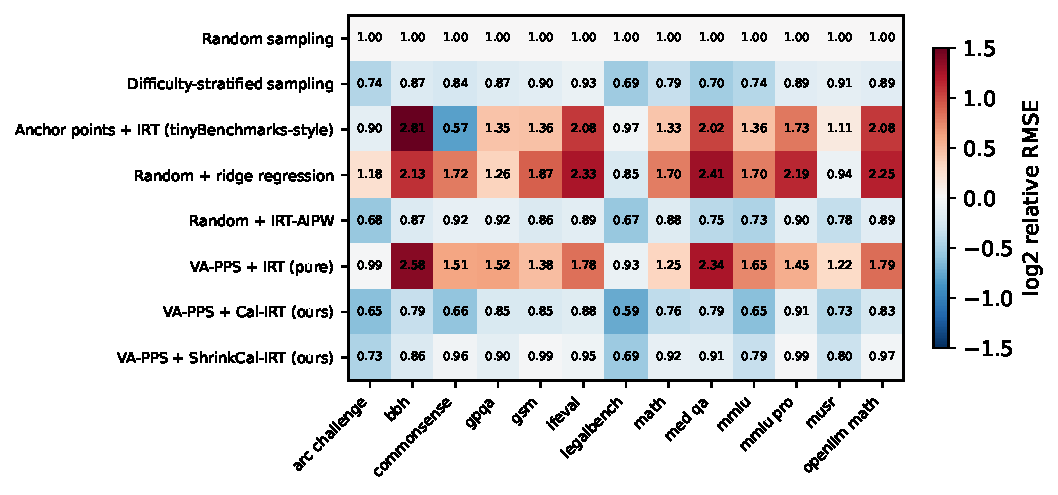
\includegraphics[width=0.95\linewidth]{figs/perbench_top100.pdf}
\caption{Per-benchmark relative RMSE at $n=100$, stronger-target split (cell values; colour = $\log_2$).}\label{fig:perbench}
\end{figure}
\begin{figure}[h]
\centering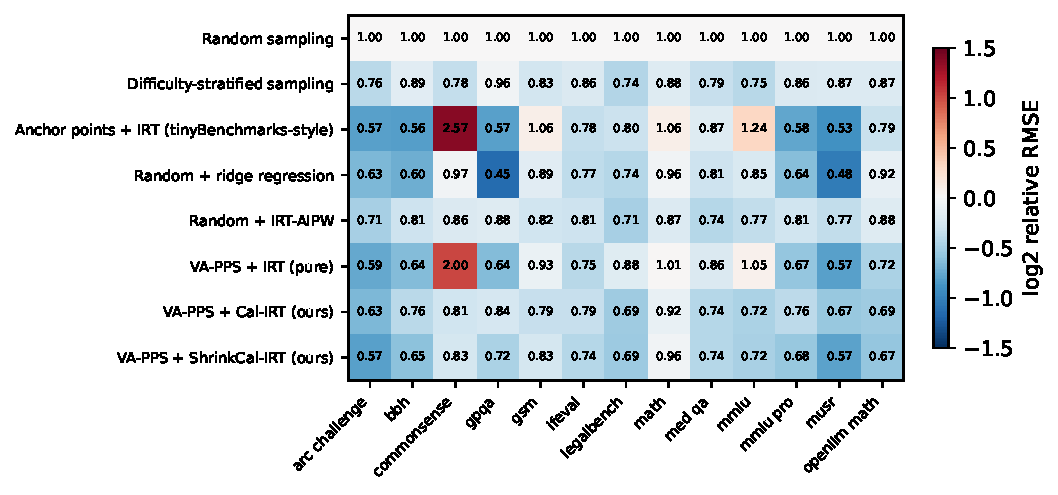
\includegraphics[width=0.95\linewidth]{figs/perbench_random100.pdf}
\caption{Per-benchmark relative RMSE at $n=100$, random split.}\label{fig:perbench2}
\end{figure}

\section{Shift severity}\label{app:shift}
Targets are the strongest 10\% / 25\% / 50\% or the weakest 25\% of models (by full-benchmark accuracy); the remaining models are sources. Ten seeds (0--9), $n\in\{25,100\}$, designs random, stratified, VA-PPS ($\lambda=1$) and anchors; the ``Stronger targets'' (25\%) column is the main-run result restricted to the same seeds.
\begin{table}[h]
\caption{Relative RMSE vs.\ random sampling under different shift severities (geometric mean over 13 benchmarks; 95\% hierarchical-bootstrap intervals).}\label{tab:shift}
\centering\tiny\setlength{\tabcolsep}{1.5pt}\resizebox{\linewidth}{!}{\begin{tabular}{lcccccccc}
\toprule
 & \multicolumn{2}{c}{Top-10\% targets} & \multicolumn{2}{c}{Stronger targets (extrapolation)} & \multicolumn{2}{c}{Top-50\% targets} & \multicolumn{2}{c}{Weakest-25\% targets} \\
 & $n$=25 & $n$=100 & $n$=25 & $n$=100 & $n$=25 & $n$=100 & $n$=25 & $n$=100 \\
\midrule
Random sampling & 1.00\,\scriptsize(1.00--1.00) & 1.00\,\scriptsize(1.00--1.00) & 1.00\,\scriptsize(1.00--1.00) & 1.00\,\scriptsize(1.00--1.00) & 1.00\,\scriptsize(1.00--1.00) & 1.00\,\scriptsize(1.00--1.00) & 1.00\,\scriptsize(1.00--1.00) & 1.00\,\scriptsize(1.00--1.00) \\
Difficulty-stratified sampling & 0.88\,\scriptsize(0.81--0.97) & 0.77\,\scriptsize(0.69--0.86) & 0.82\,\scriptsize(0.75--0.90) & 0.81\,\scriptsize(0.74--0.88) & 0.86\,\scriptsize(0.80--0.93) & 0.81\,\scriptsize(0.74--0.90) & 0.92\,\scriptsize(0.84--1.00) & 0.90\,\scriptsize(0.84--0.98) \\
Anchor points + IRT (tinyBenchmarks-style) & 0.96\,\scriptsize(0.80--1.19) & 1.00\,\scriptsize(0.74--1.30) & 1.02\,\scriptsize(0.85--1.24) & 1.37\,\scriptsize(1.09--1.74) & 1.34\,\scriptsize(1.11--1.67) & 1.97\,\scriptsize(1.61--2.50) & 1.36\,\scriptsize(0.98--1.87) & 2.16\,\scriptsize(1.47--3.15) \\
Random + ridge regression & 1.12\,\scriptsize(0.95--1.32) & 1.24\,\scriptsize(1.08--1.47) & 1.13\,\scriptsize(0.93--1.38) & 1.60\,\scriptsize(1.33--1.98) & 1.43\,\scriptsize(1.16--1.81) & 2.13\,\scriptsize(1.75--2.67) & 1.48\,\scriptsize(1.02--2.07) & 2.09\,\scriptsize(1.41--3.05) \\
Random + IRT-AIPW & 0.82\,\scriptsize(0.76--0.92) & 0.71\,\scriptsize(0.66--0.79) & 0.78\,\scriptsize(0.71--0.87) & 0.84\,\scriptsize(0.78--0.91) & 0.83\,\scriptsize(0.75--0.93) & 0.82\,\scriptsize(0.75--0.89) & 0.93\,\scriptsize(0.84--1.03) & 0.95\,\scriptsize(0.88--1.02) \\
VA-PPS + IRT (pure) & 1.00\,\scriptsize(0.84--1.22) & 1.16\,\scriptsize(1.04--1.36) & 1.03\,\scriptsize(0.87--1.25) & 1.48\,\scriptsize(1.28--1.77) & 1.33\,\scriptsize(1.11--1.62) & 2.07\,\scriptsize(1.77--2.49) & 1.38\,\scriptsize(1.00--1.84) & 2.12\,\scriptsize(1.50--2.99) \\
VA-PPS + Cal-IRT (ours) & 0.72\,\scriptsize(0.63--0.82) & 0.68\,\scriptsize(0.61--0.76) & 0.71\,\scriptsize(0.62--0.81) & 0.73\,\scriptsize(0.67--0.81) & 0.84\,\scriptsize(0.76--0.95) & 0.82\,\scriptsize(0.71--0.95) & 0.90\,\scriptsize(0.77--1.06) & 0.92\,\scriptsize(0.81--1.05) \\
VA-PPS + ShrinkCal-IRT (ours) & 0.83\,\scriptsize(0.72--0.98) & 0.80\,\scriptsize(0.73--0.91) & 0.81\,\scriptsize(0.71--0.94) & 0.85\,\scriptsize(0.79--0.93) & 0.95\,\scriptsize(0.84--1.09) & 0.93\,\scriptsize(0.82--1.07) & 1.01\,\scriptsize(0.84--1.20) & 1.07\,\scriptsize(0.93--1.24) \\
\bottomrule
\end{tabular}
}
\end{table}
\begin{table}[h]
\caption{Mean signed error (accuracy points, averaged over benchmarks) and bias$^2$/MSE at $n=100$ under different shifts.}\label{tab:shiftbias}
\centering\tiny\setlength{\tabcolsep}{1.5pt}\resizebox{\linewidth}{!}{\begin{tabular}{lcccccccc}
\toprule
 & \multicolumn{2}{c}{Top-10\% targets} & \multicolumn{2}{c}{Stronger targets (extrapolation)} & \multicolumn{2}{c}{Top-50\% targets} & \multicolumn{2}{c}{Weakest-25\% targets} \\
 & mean err (pts) & bias$^2$/MSE & mean err (pts) & bias$^2$/MSE & mean err (pts) & bias$^2$/MSE & mean err (pts) & bias$^2$/MSE \\
\midrule
Random sampling & -0.07 & 55\% & -0.55 & 41\% & -0.07 & 45\% & +0.04 & 26\% \\
Difficulty-stratified sampling & +0.10 & 26\% & -0.15 & 18\% & -0.12 & 16\% & -0.13 & 11\% \\
Anchor points + IRT (tinyBenchmarks-style) & -3.81 & 74\% & -5.01 & 72\% & -7.51 & 70\% & +9.01 & 70\% \\
Random + ridge regression & -4.43 & 81\% & -5.58 & 76\% & -7.99 & 73\% & +8.15 & 67\% \\
Random + IRT-AIPW & -0.20 & 17\% & -0.33 & 19\% & -0.31 & 21\% & +0.21 & 22\% \\
VA-PPS + IRT (pure) & -4.08 & 78\% & -5.17 & 76\% & -7.58 & 73\% & +8.23 & 69\% \\
VA-PPS + Cal-IRT (ours) & -0.63 & 25\% & -0.41 & 16\% & -0.74 & 24\% & +1.31 & 25\% \\
VA-PPS + ShrinkCal-IRT (ours) & -1.62 & 40\% & -1.44 & 29\% & -1.79 & 35\% & +2.28 & 40\% \\
\bottomrule
\end{tabular}
}
\end{table}


\section{Number of source models}\label{app:src}
Seven benchmarks (ARC-Challenge, GPQA, IFEval, MuSR, MATH Lvl 5, HELM MMLU, HELM GSM), seeds 0--9; $m$ source models drawn at random from the split's source set (``all'' = no subsampling; HELM splits have fewer than 100 sources, so $m=100$ equals ``all'' there). Relative RMSE vs.\ random sampling on the same targets (random sampling does not depend on $m$).
\begin{table}[h]
\caption{Relative RMSE vs.\ number of source models $m$, $n=25$.}\label{tab:src25}
\centering\tiny\setlength{\tabcolsep}{1.5pt}\resizebox{\linewidth}{!}{\begin{tabular}{lcccccccc}
\toprule
 & \multicolumn{4}{c}{Random split} & \multicolumn{4}{c}{Stronger targets} \\
 & $m$=20 & $m$=50 & $m$=100 & $m$=all & $m$=20 & $m$=50 & $m$=100 & $m$=all \\
\midrule
Difficulty-stratified sampling & 0.82\,\scriptsize(0.74--0.91) & 0.84\,\scriptsize(0.75--0.94) & 0.82\,\scriptsize(0.74--0.91) & 0.80\,\scriptsize(0.72--0.90) & 0.79\,\scriptsize(0.70--0.89) & 0.80\,\scriptsize(0.68--0.91) & 0.79\,\scriptsize(0.69--0.90) & 0.79\,\scriptsize(0.70--0.89) \\
VA-PPS + ridge regression & 0.71\,\scriptsize(0.52--0.95) & 0.56\,\scriptsize(0.42--0.74) & 0.52\,\scriptsize(0.38--0.70) & 0.51\,\scriptsize(0.37--0.69) & 1.22\,\scriptsize(0.88--1.70) & 1.05\,\scriptsize(0.75--1.47) & 0.97\,\scriptsize(0.70--1.30) & 0.96\,\scriptsize(0.70--1.30) \\
VA-PPS + IRT (pure) & 0.77\,\scriptsize(0.55--1.02) & 0.61\,\scriptsize(0.46--0.79) & 0.55\,\scriptsize(0.43--0.72) & 0.56\,\scriptsize(0.43--0.72) & 1.47\,\scriptsize(1.04--2.06) & 1.14\,\scriptsize(0.83--1.55) & 1.01\,\scriptsize(0.75--1.31) & 0.87\,\scriptsize(0.69--1.12) \\
VA-PPS + IRT-AIPW & 0.96\,\scriptsize(0.80--1.15) & 0.82\,\scriptsize(0.70--0.97) & 0.71\,\scriptsize(0.62--0.82) & 0.73\,\scriptsize(0.63--0.84) & 1.51\,\scriptsize(0.92--2.06) & 0.97\,\scriptsize(0.66--1.37) & 0.84\,\scriptsize(0.63--1.11) & 0.79\,\scriptsize(0.65--0.96) \\
VA-PPS + Cal-IRT & 0.71\,\scriptsize(0.58--0.86) & 0.65\,\scriptsize(0.54--0.77) & 0.63\,\scriptsize(0.53--0.74) & 0.64\,\scriptsize(0.54--0.75) & 0.86\,\scriptsize(0.67--1.07) & 0.76\,\scriptsize(0.61--0.95) & 0.74\,\scriptsize(0.60--0.91) & 0.68\,\scriptsize(0.56--0.81) \\
VA-PPS + ShrinkCal-IRT & 0.70\,\scriptsize(0.54--0.88) & 0.62\,\scriptsize(0.50--0.75) & 0.57\,\scriptsize(0.46--0.69) & 0.58\,\scriptsize(0.47--0.71) & 0.98\,\scriptsize(0.77--1.22) & 0.87\,\scriptsize(0.67--1.10) & 0.81\,\scriptsize(0.64--0.98) & 0.73\,\scriptsize(0.59--0.91) \\
\bottomrule
\end{tabular}
}
\end{table}
\begin{table}[h]
\caption{Relative RMSE vs.\ number of source models $m$, $n=100$.}\label{tab:src100}
\centering\tiny\setlength{\tabcolsep}{1.5pt}\resizebox{\linewidth}{!}{\begin{tabular}{lcccccccc}
\toprule
 & \multicolumn{4}{c}{Random split} & \multicolumn{4}{c}{Stronger targets} \\
 & $m$=20 & $m$=50 & $m$=100 & $m$=all & $m$=20 & $m$=50 & $m$=100 & $m$=all \\
\midrule
Difficulty-stratified sampling & 0.86\,\scriptsize(0.78--0.96) & 0.83\,\scriptsize(0.76--0.91) & 0.85\,\scriptsize(0.77--0.93) & 0.83\,\scriptsize(0.75--0.91) & 0.83\,\scriptsize(0.73--0.92) & 0.82\,\scriptsize(0.74--0.90) & 0.84\,\scriptsize(0.77--0.93) & 0.83\,\scriptsize(0.74--0.92) \\
VA-PPS + ridge regression & 0.92\,\scriptsize(0.75--1.10) & 0.75\,\scriptsize(0.62--0.89) & 0.75\,\scriptsize(0.61--0.91) & 0.66\,\scriptsize(0.53--0.82) & 1.96\,\scriptsize(1.43--2.81) & 1.71\,\scriptsize(1.30--2.30) & 1.60\,\scriptsize(1.25--2.12) & 1.42\,\scriptsize(1.10--1.83) \\
VA-PPS + IRT (pure) & 1.25\,\scriptsize(1.00--1.49) & 0.86\,\scriptsize(0.72--1.01) & 0.80\,\scriptsize(0.66--0.95) & 0.71\,\scriptsize(0.61--0.83) & 2.63\,\scriptsize(1.98--3.70) & 1.96\,\scriptsize(1.48--2.62) & 1.70\,\scriptsize(1.34--2.18) & 1.40\,\scriptsize(1.20--1.60) \\
VA-PPS + IRT-AIPW & 1.12\,\scriptsize(1.00--1.24) & 0.85\,\scriptsize(0.73--1.00) & 0.83\,\scriptsize(0.74--0.93) & 0.78\,\scriptsize(0.69--0.89) & 1.16\,\scriptsize(0.92--1.51) & 0.96\,\scriptsize(0.74--1.24) & 0.87\,\scriptsize(0.73--1.04) & 0.82\,\scriptsize(0.69--0.96) \\
VA-PPS + Cal-IRT & 0.84\,\scriptsize(0.71--0.95) & 0.75\,\scriptsize(0.65--0.84) & 0.76\,\scriptsize(0.67--0.85) & 0.73\,\scriptsize(0.65--0.82) & 0.94\,\scriptsize(0.75--1.22) & 0.85\,\scriptsize(0.70--1.04) & 0.81\,\scriptsize(0.65--1.00) & 0.73\,\scriptsize(0.63--0.83) \\
VA-PPS + ShrinkCal-IRT & 0.86\,\scriptsize(0.74--0.97) & 0.71\,\scriptsize(0.61--0.82) & 0.72\,\scriptsize(0.62--0.84) & 0.68\,\scriptsize(0.60--0.77) & 1.10\,\scriptsize(0.92--1.34) & 0.95\,\scriptsize(0.83--1.12) & 0.90\,\scriptsize(0.75--1.07) & 0.82\,\scriptsize(0.73--0.93) \\
\bottomrule
\end{tabular}
}
\end{table}

\section{Reproducibility and disclosures}\label{app:repro}
\textbf{Code and commands.} See \texttt{README.md} in the supplementary code. In short: \texttt{run\_exp.py --tag main --seeds 0-29 --budgets 10,25,50,100,200 --auto --jobs 4} (main grid, 990 jobs, about 3.5\,h on 4 CPU cores), \texttt{run\_exp.py --tag shift --protocols top10,top50,bottom --seeds 0-9 --budgets 25,100 --designs rand,strat,pps1.0,anchor} (shift-severity run), and the source-size runs (\texttt{run\_exp.py --tag src$K$ --benchmarks arc\_challenge,gpqa,ifeval,musr,openllm\_math,mmlu,gsm --protocols random,top --seeds 0-9 --budgets 25,100 --designs strat,pps1.0 --max\_sources $K$}, $K\in\{20,50,100\}$); then \texttt{analyze.py main}, \texttt{analyze.py shift} and \texttt{analyze\_src.py} regenerate all tables and figures. Re-running two main-grid jobs (IFEval and GSM, stronger-target split, seed 3) reproduced all stored results exactly (maximum absolute difference 0). Software: Python 3.11, numpy 2.4.6, scipy 1.17.1, scikit-learn 1.9.1, pandas 3.1.0, joblib 1.6.0, matplotlib 3.11.2. Randomness: split seed $s$ uses \texttt{default\_rng(10000+s)}; coreset/IRT-initialisation randomness uses \texttt{default\_rng(s)}; AUTO inner splits use \texttt{default\_rng(777000+s)}. Development runs used seeds $\ge1000$ (and 2000--2007) and are not part of the reported tables.\\
\textbf{Data.} Files \texttt{data/scores/*.jbl} from \url{https://github.com/socialfoundations/benchmark-prediction} at commit \texttt{55faff496947789f94e6b5908c77cbc3e84f81ad} (SHA-256 sums of all files are recorded in \texttt{data/SHA256SUMS.txt}). We only used the score matrices and model lists; we did not use the \texttt{benchpred} package, nor re-run any model. Upstream sources: Open LLM Leaderboard v2, HELM.\\
\textbf{Related-work disclosure.} Regarding the restriction on reading the paper that studies this exact problem: we did not search for, open or read any paper on that topic apart from the items of the provided starter list. The starter list includes the NeurIPS 2025 paper of \citet{zhang2025misses}; we did \emph{not} read it. Our knowledge of it is limited to its description in the starter list and the README of the data repository (which we read when downloading the data and which summarises its conclusions in three sentences, quoted in spirit in Section~\ref{sec:related}). Other literature was located through a scholarly-search tool (titles and abstract snippets only) to verify citation details. No other encounter with restricted content occurred.\\
\textbf{Use of an AI agent.} All code, experiments, analysis and text of this study were produced by an autonomous AI research agent (Claude Sonnet 5.5, Claude Agent SDK) running unattended.\\
\textbf{Failed or abandoned items.} The first launch of the main run used 38 worker processes under a 4-core CPU quota and was killed and restarted with 4 workers before producing any result file. The cross-fitted AIPW variant (\texttt{gregcf}) was worse than in-sample AIPW and is reported in Table~\ref{tab:abl} only. On the development run, weaker item regularisation (0.2 instead of 1) was slightly worse for Cal-IRT and larger ability-prior variances (25, 1000) were similar or worse, so neither was adopted; extra Platt penalties (5, 20) and an intercept-only recalibration were not better than the default either.
